\section{Single Specie Methods}
A system of equations suitable for solution via iterative methods is now presented for solving the straight-ahead equation,
which, in operator notation, is 
%
\begin{equation} 
  \label{eqn:fpe-e-2}
  \left(\bA{L} - \bA{C} - \bA{T} \right) \vec{\Psi} = \vec{q},
\end{equation}
%
where $\bA{L}$ is the spatial streaming operator, $\bA{C}$ is the CSD operator,
and $\bA{T}$ is the energy-straggling operator.
This new system of equations is found by splitting the operators in \ref{eqn:fpe-e-2}
into lower or upper triangular parts that can be easily inverted, and multiplying \ref{eqn:fpe-e-2} from the left by inverses of the split upper or lower triangular operators. This new split system of equations will be closer to the identity matrix
than the original, un-split, system of equations and will converge more rapidly to the solution improving the overall time-to-solution.

To begin the energy operators $\bA{C}$ and $\bA{T}$ are split into lower and upper triangular pieces. Note, because of the energy group ordering, low to high, the split lower-triangular and upper-triangular operators will describe up-scattering and down-scattering in energy respectively. The energy-straggling operator, which allows for both up-scatter and down-scatter, is split into lower and upper triangular parts, that is,
\[
  \bA{T} = \bA{T}_{\text{L}} + \bA{T}_{\text{U}},
\]
where the subscripts L and U represent the lower and upper-triangular parts respectively. The continuous slowing down operator $\bA{C}$ only allows particles to down-scatter in energy and is therefore upper-triangular in energy. Summing the upper-triangular operators $\bA{T}_{\text{U}}$ and $\bA{C}$ results in an operator that is upper-triangular in energy and block diagonal in space,
\[
  \bA{F} = \bA{C} + \bA{T}_{\text{U}}.
\]
The operator $\bA{F}$ can be easily inverted by \emph{sweeping} from high-to-low across the energy domain, and \emph{sweeping} from either left-to-right or right-to-left across the spatial domain. Here \emph{sweeping} refers to the action of starting from the boundary of the problem and moving with the direction of particle flow across the entire domain solving the system of equations for a given space-energy cell $I_{i,g}$ using the upwinding from the previous cell.

The \dG spatial discretization results in $\bA{L}$ being lower-triangular in space and block diagonal in energy. Therefore, $\bA{L}$ can be easy inverted by \emph{sweeping} from left-to-right across the spatial domain and \emph{sweeping} either from low-to-high or high-to-low across the energy domain. Summing $\bA{L}$ and $\bA{F}$ results in an operator that is lower-triangular in space and upper-triangular in energy, whose inverse can be efficiently found by \emph{sweeping} from left-to-right across the spatial domain while simultaneously \emph{sweeping} from high-to-low across the energy domain. 

The new system of equations that results from this splitting is found by multiplying \ref{eqn:fpe-e-2} from the left by the inverse of the sum of $\bA{L}$ and $\bA{F}$, that is, 
\begin{equation} 
  \label{eqn:system-M1}
  \left\lbrace \bA{I} - \Big[ \bA{L} - \bA{F} \Big]^{-1} \bA{T}_{\text{L}} \right\rbrace \vec{\Psi}
  = \Big[ \bA{L} - \bA{F} \Big]^{-1} \vec{q},
\end{equation}
where $\bA{I}$ is the identity operator. Iterative solutions to \ref{eqn:system-M1} will converge quickly provided that $\bA{T}_{\text{L}}$ does not dominate the problem,
that is, if the spectrum of $\bA{T}_{\text{L}}$
is ``small'', such that the overall spectrum of \ref{eqn:system-M1} is ``small''. However, being a differential operator, the spectrum of $\bA{T}_{\text{L}}$ might be so large that it overwhelms the contraction effected by the action of $[\bA{L} - \bA{F}]^{-1}$, but this is problem dependent.

A simple fixed-point iteration that corresponds to \ref{eqn:system-M1} lags $\bA{T}_{\text{L}}$, that is,
\begin{equation}
  \label{eqn:jacobi_A4}
  x^{l+1} = \big[\bA{L} - \bA{F} \big]^{-1} \left( \bA{T}_{\text{L}} x^{l} + b \right), \quad l=0,1,2,\ldots
\end{equation}
where $l$ is the iteration index. Algorithm \ref{eqn:jacobi_A4} will converge if all the eigenvalues of the operator $[\bA{L} - \bA{F}]^{-1}$ are less-than one in magnitude. Additionally, \ref{eqn:jacobi_A4} will converge rapidly if the magnitude of all the eigenvalues of $[\bA{L} - \bA{F}]^{-1}$ are close to zero, as the closer to one in magnitude the slower converging the system of equations will be. 

% -------------------------------------------------------------------------
% Numerical Algorithm Experiments
% -------------------------------------------------------------------------
\subsection{Numerical Algorithm Experiments}
To investigate the efficiency of iterative numerical methods at solving \ref{eqn:system-M1}, the following charged particle transport problem is investigated. The problem consists of a volume source of alpha-particles in a deuterium-tritium (DT) gas next to slabs of DT ice and high-density-Carbon (HDC). Figure \ref{fig:deuteron_problem} shows the geometric layout and material properties of the problem which are similar to the DT pellets used by the National Ignition Facility in ICF experiments \cite{Lindl-2018}\cite{Pape-2018}. The volume source of alpha-particles in the DT region of the problem is
\begin{equation}
  \label{eqn:alpha-volume-source}
  q(x,E) = 
  \begin{cases}
    10^{13} \left[1 - \left(\dfrac{x}{0.1 \cm}\right)^2 \right] \exp\left[\frac{1}{2 \sigma^2}(E - \mu)^2 \right], \quad &\text{for} \, x \in [0,0.0792 \cm], \\
    0, \quad\quad &\text{otherwise},
  \end{cases}
\end{equation}
where $\mu=3.5 \mev$, and $\sigma = 0.01 \mev$. Additionally, because \ref{eqn:alpha-volume-source} is not zero at the left boundary of the problem a boundary source on the left-hand boundary of the problem is required, that is,
\begin{equation}
  f(E) = 10^{13} \exp\left[\frac{1}{2 \sigma^2}(E - \mu)^2 \right].
\end{equation}

\begin{figure}[!htb]
  \centering
  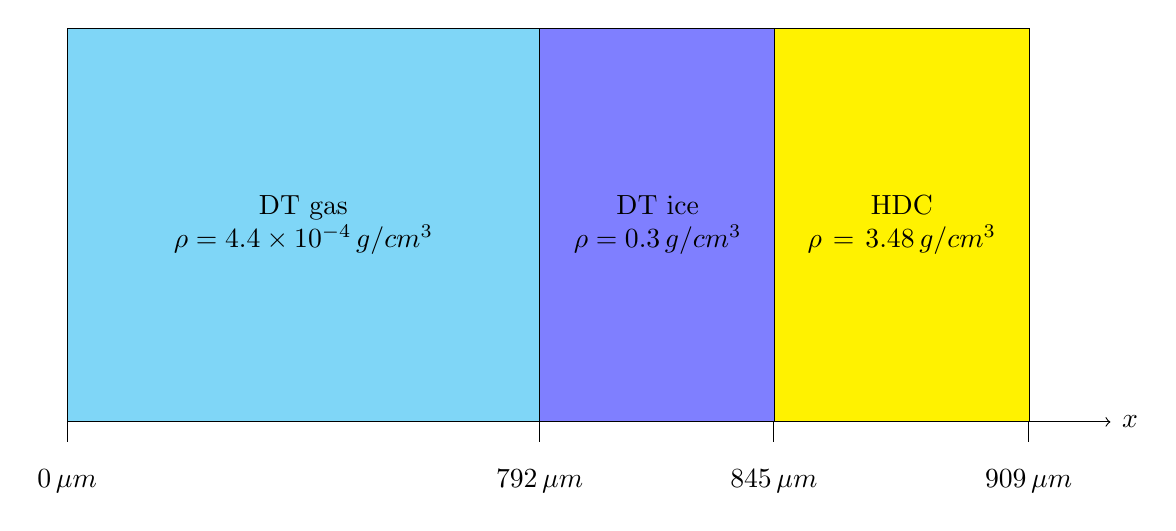
\begin{tikzpicture}
    \node[rectangle, draw = black,
          text = black,
          fill = cyan,
          fill opacity = 0.5,
          text opacity = 1.0,
          minimum width = 6cm, 
          align=center,
          minimum height = 5cm] (r1) at (-4.75,0) {DT gas\\$\rho = 4.4 \times 10^{-4} \,\text{g}/\text{cm}^3$};
    \node[rectangle, draw = black,
          text = black,
          fill = blue,
          fill opacity = 0.5,
          text opacity = 1.0,
          minimum width = 3.0cm,
          align=center, 
          minimum height = 5cm] (r2) at (-0.25,0) {DT ice\\$\rho = 0.3\,\text{g}/\text{cm}^3$};
    \node[rectangle, draw = black,
          text = black,
          fill = yellow,
          align=center,
          minimum width = 3cm,
          text width = 3cm, 
          minimum height = 5cm] (r3) at ( 2.85,0) {HDC\\$\rho = 3.48\,\text{g}/\text{cm}^3$};
    \node[draw=white] at (-7.75,-3.25) {$0 \, \mu \text{m}$};
    \node[draw=white] at (-1.75,-3.25) {$792 \, \mu \text{m}$};
    \node[draw=white] at ( 1.225,-3.25) {$845 \, \mu \text{m}$};
    \node[draw=white] at ( 4.46,-3.25) {$909 \, \mu \text{m}$};

    \draw (-7.75,-2.5) -- (-7.75,-2.75);
    \draw (-1.75,-2.5) -- (-1.75,-2.75);
    \draw ( 1.225,-2.5) -- ( 1.225,-2.75);
    \draw ( 4.46,-2.5) -- ( 4.46,-2.75);
    \draw[->] (-6,-2.5) -- (5.5,-2.5);
    \node[draw=white] at ( 5.75,-2.5) {$x$};
  \end{tikzpicture}
  \caption{Geometry of the problem}
  \label{fig:deuteron_problem}  
\end{figure}

The problem is discretized in energy using both the alternating flux and ``directional flows'' \dGn{2} methods on a $256$ group evenly spaced energy grid. The spatial domain is discretized using a \dGn{2} method with $86$, $85$, and $85$ evenly spaced spatial cells in the DT gas, DT ice, and HDC spatial regions of the problem. To describe the ion-nucleus interactions that the alpha-particles experience, the nuclear stopping powers and energy-straggling coefficients corresponding to the Wentzel-Moli\`{e}re differential cross section are used. The Wentzel-Moli\`{e}re differential cross section describes the interactions of charged particles with cold nuclei as they slow down in materials \cite{boschini-2011}. The interactions between the alpha-particles and the background electrons are described by electronic stopping powers and energy-straggling coefficients that correspond to the relativistic Rutherford differential cross section. The relativistic Rutherford differential cross section describes collisions between ions and free electrons in cold materials \cite{evans-1976}. The multigroup stopping power and energy-straggling coefficients required by the \dG discretizations are calculated as,
\begin{eqnarray}
  S_g = \dfrac{\int_{I_g} dE \, w(E) \, S(E)}{\int_{I_g} dE \, w(E)}, \quad T_g = \dfrac{\int_{I_g} dE \, w(E) \, T(E)}{\int_{I_g} dE \, w(E)}
\end{eqnarray}
where $w(E)$ is the weighting function taken in this work to be a constant. 

It was observed that the systems of equations were non-symmetric, non-normal and, in general not symmetric-positive-definite meaning that Krylov iterative methods suitable for non-symmetric systems of equations are needed to solve \ref{eqn:system-M1}. The Krylov iterative methods used are the restarted generalized minimum residual method (GMRES(m)) method, and the bi-conjugate gradient stabilized method (BiCGStab). Additionally, it was observed that the eigenvalues of the inverse of $\bA{L} - \bA{F}$ were all less than one in magnitude, and to that end the systems of equations were solved using the fixed point Jacobi iteration method. To compare the efficiency of the iterative methods at solving the two \dG systems of equations, the number of matrix-vector multiplications required by each iterative method to converge to the desired tolerance are compared. For the GMRES(p) and Jacobi iterative methods the number of matrix-vector multiplications is simply the number of iterations required to converge the relative residual to a fixed tolerance. However, because BiCGStab requires the application of the operator twice per iteration, the total number of matrix-vector multiplications required by BiCGStab is twice the number of iterations required to converge the relative residual to a fixed tolerance.

Table \ref{tab:alpha_particle} shows the number of matrix-vector multiplications required by the iterative methods to converge the relative residual to a tolerance of $10^{-12}$. From Table \ref{tab:alpha_particle}, the system of equations that results from the alternating flux \dG discretization results in a system that can be solved in significantly fewer matrix-vector multiplications than the equivalent ``directional flows'' system of equations. Additionally, the alternating flux system of equations can be solved using GMRES(p) with a small restart whereas the ``directional flows'' system of equations requires a large restart for GMRES(p). The fixed point Jacobi iteration method converges quickly for the alternating flux method suggesting that the eigenvalues of the inverse of $\bA{L} - \bA{F}$ are close to zero in magnitude, which is desirable by fixed point methods. Using Jacobi iteration, the ``directional flows'' system of equations is very slow to converge suggesting that the inverse of $\bA{L} - \bA{F}$ has a significant number of eigenvalues near one.

\begin{table}[!htb]
  \centering
  \caption{Number of matrix-vector multiplications required by the iterative methods to converge to relative residual $10^{-12}$}
  \begin{tabular}{c|c|c}
    \toprule
    Iterative Method     & alternating flux & ``directional flows'' \\
    \midrule
    GMRES(5)   & 21               & 410               \\
    GMRES(10)  & 20               & 150               \\
    GMRES(15)  & 19               & 131               \\
    GMRES(20)  & 19               & 121               \\
    GMRES(25)  & 19               & 117               \\
    Full GMRES & 19               & 105               \\
    BiCGStab   & 20               & 184               \\
    Jacobi     & 28               & 4873              \\
    \bottomrule
  \end{tabular}
  \label{tab:alpha_particle}
\end{table}

In Figure \ref{fig:eigen_spectra_alpha} the eigenvalue spectra of the equivalent $32 \times 32$ \dGn{1} alternating flux and ``directional flows'' systems of equations for the alpha-particle problem are shown. From Figure \ref{fig:eigen_spectra_alpha} the eigenvalue spectrum of the alternating flux system of equations is significantly more compact than the eigenvalue spectrum of the ``directional flows'' system of equations meaning that iterative Krylov methods will be more efficient at solving the alternating flux system of equations in comparison to the ``directional flows'' system. This efficiency reflected in Table \ref{tab:alpha_particle} by the number of matrix-vector multiplications being significantly less for the alternating flux than the ``directional flows'' systems of equations.

\begin{figure}[!htb]
  \centering
  \begin{subfigure}{.45\textwidth}
    \centering
    \includegraphics[width=\linewidth]{figures/chapter-7/eig_alphas_A4_af.pdf}
    \caption{alternating flux}
    \label{fig:eigen_spectra_alpha_af}
  \end{subfigure}
  \begin{subfigure}{.45\textwidth}
    \centering
    \includegraphics[width=\linewidth]{figures/chapter-7/eig_alphas_A4_df.pdf}
    \caption{``directional flows''}
    \label{fig:eigen_spectra_alpha_df}
  \end{subfigure}
  \caption{Eigenvalue spectra for the alternating flux and ``directional flows'' \dG systems of equations} 
  \label{fig:eigen_spectra_alpha}
\end{figure}